% !TEX encoding = UTF-8 Unicode
% !TEX TS-program = xelatex
\begin{QUESTIONS}
    \begin{QUESTION}
        \begin{ExamInfo}{91}{學測}{單選}{1}
        \end{ExamInfo}
        \begin{ExamAnsRateInfo}{76}{97}{83}{48}
        \end{ExamAnsRateInfo}
        \begin{QBODY}
            設 $P(x,y)$ 為坐標平面上一點,且滿足
            $(x-1)^2 +(y-2)^2 + (x-3)^2 +(y-4)^2 = (3-1)^2 +(4-2)^2$
            ,那麼 $P$ 點的位置在哪裡?
            
            \begin{QOPS} 
                \QOP 第一象限 
                \QOP 第二象限 
                \QOP 第三象限 
                \QOP 第四象限 
                \QOP $x$ 軸或 $y$ 軸上
            \end{QOPS}
        \end{QBODY}
        \begin{QFROMS}
        \end{QFROMS}
        \begin{QTAGS}\QTAG{B3C2-1直線方程式及其圖形}\QTAG{B3C2直線與圓}\end{QTAGS}
        \begin{QANS}
            (1)
        \end{QANS}
        \begin{QSOLLIST}
        \end{QSOLLIST}
        \begin{QEMPTYSPACE}
        \end{QEMPTYSPACE}
    \end{QUESTION}
    \begin{QUESTION}
        \begin{ExamInfo}{91}{學測}{單選}{2}
        \end{ExamInfo}
        \begin{ExamAnsRateInfo}{51}{79}{51}{23}
        \end{ExamAnsRateInfo}
        \begin{QBODY}
            一群登山友,在山上發現一顆巨樹,隊中 $10$ 位身高 $170$ 公分的男生,手拉著手剛好環抱大樹一 圈。問樹幹的直徑最接近下列何值? 
            \begin{QOPS} 
                \QOP $3$公尺 
                \QOP $5$公尺
                \QOP $7$公尺 
                \QOP $9$公尺 
                \QOP $11$ 公尺
            \end{QOPS}
        \end{QBODY}
        \begin{QFROMS}
        \end{QFROMS}
        \begin{QTAGS}\QTAG{不是99課綱}\end{QTAGS}
        \begin{QANS}
            (2)
        \end{QANS}
        \begin{QSOLLIST}
        \end{QSOLLIST}
        \begin{QEMPTYSPACE}
        \end{QEMPTYSPACE}
    \end{QUESTION}
    \begin{QUESTION}
        \begin{ExamInfo}{91}{學測}{單選}{3}
        \end{ExamInfo}
        \begin{ExamAnsRateInfo}{62}{94}{65}{27}
        \end{ExamAnsRateInfo}
        \begin{QBODY}
            如圖,下面哪一選項中的向量與另兩個向量 $\lvec{PO}$, $\lvec{QO}$ 之和等於零向量?
            \begin{QOPS} 
                \QOP $\lvec{AO}$ 
                \QOP $\lvec{BO}$ 
                \QOP $\lvec{CO}$ 
                \QOP $\lvec{DO}$ 
                \QOP $\lvec{EO}$ 
            \end{QOPS}

                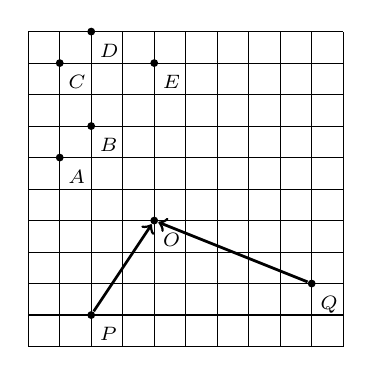
\begin{tikzpicture}[scale=.4]
                \draw (0,0) grid (10,10);\scriptsize
                \foreach \v/\x/\y in {P/2/1,Q/9/2,O/4/4,A/1/6,B/2/7,C/1/9,D/2/10,E/4/9}
                \node[fill,inner sep=1pt,circle] (v\v) at (\x,\y)[label=280:$\v$] {};
                \foreach \i/\j in {P/O, Q/O}
                \draw[->,line width=1pt] (v\i) to (v\j);
                \end{tikzpicture}
        \end{QBODY}
        \begin{QFROMS}
        \end{QFROMS}
        \begin{QTAGS}\QTAG{線性組合}\QTAG{B3C3-1平面向量的表示法}\QTAG{B3C3平面向量}\end{QTAGS}
        \begin{QANS}
            (3)
        \end{QANS}
        \begin{QSOLLIST}
        \end{QSOLLIST}
        \begin{QEMPTYSPACE}
        \end{QEMPTYSPACE}
    \end{QUESTION}
    \begin{QUESTION}
        \begin{ExamInfo}{91}{學測}{單選}{4}
        \end{ExamInfo}
        \begin{ExamAnsRateInfo}{35}{60}{27}{18}
        \end{ExamAnsRateInfo}
        \begin{QBODY}
            若某校 $1000$ 位學生的數學段考成績平均分數是 $65.24$ 分,樣本標準差是 $5.24$ 分,而且已知成績分佈呈現常態分配。試問全校約有多少人數學成績低於 $60$ 分?
            \begin{QOPS}
                \QOP 約$80$人  
                \QOP 約$160$人 
                \QOP 約$240$人 
                \QOP 約$320$人 
                \QOP 約$400$人
            \end{QOPS}
        \end{QBODY}
        \begin{QFROMS}
        \end{QFROMS}
        \begin{QTAGS}\QTAG{B5C1機率與統計}\QTAG{B5C1-3抽樣與統計推論}\end{QTAGS}
        \begin{QANS}
            (2)
        \end{QANS}
        \begin{QSOLLIST}
        \end{QSOLLIST}
        \begin{QEMPTYSPACE}
        \end{QEMPTYSPACE}
    \end{QUESTION}
    \begin{QUESTION}
        \begin{ExamInfo}{91}{學測}{單選}{5}
        \end{ExamInfo}
        \begin{ExamAnsRateInfo}{52}{82}{54}{20}
        \end{ExamAnsRateInfo}
        \begin{QBODY}
            試問用下列哪一個函數的部分圖形來描述右圖較恰當?
            \begin{QOPS}
            \QOP $(x-2)^{2}-2$  
            \QOP $2\sin(x)+2$
            \QOP $2\cos(x)$ 
            \QOP $-0.5(x-2)^{2}+4$ 
            \QOP $3-2^{x}$ 
            \end{QOPS}
            \begin{tikzpicture}[scale=.5]
                \begin{scope}\scriptsize
                \draw[->] (0,-1) to (0,5) node[above] {$y$};
                \draw[->] (-1,0) to (5,0) node[right] {$x$};
                \node[] at (1,-.6) {$(1,0)$};
                \node[] at (-1,1) {$(0,1)$};
                \node[draw,fill,circle,inner sep=1pt] at (0,1) {};
                \node[draw,fill,circle,inner sep=1pt] at (1,0) {};
                \draw[smooth,samples=100,domain=0:5] plot(\x,{-.5*(\x-2)*(\x-2)+4});
                %\draw[smooth,samples=100] (3,3) ellipse (2cm and 4cm) ;
                \end{scope}
            \end{tikzpicture}
        \end{QBODY}
        \begin{QFROMS}
        \end{QFROMS}
        \begin{QTAGS}\QTAG{跨章節試題}\end{QTAGS}
        \begin{QANS}
            (4)
        \end{QANS}
        \begin{QSOLLIST}
        \end{QSOLLIST}
        \begin{QEMPTYSPACE}
        \end{QEMPTYSPACE}
    \end{QUESTION}
    \begin{QUESTION}
        \begin{ExamInfo}{91}{學測}{單選}{6}
        \end{ExamInfo}
        \begin{ExamAnsRateInfo}{33}{53}{32}{14}
        \end{ExamAnsRateInfo}
        \begin{QBODY}
            在坐標平面上有一橢圓,它的長軸落在 $x$ 軸上,短軸落在 $y$ 軸上,長軸、短軸的長度分別為 $4$、$2$。
            如圖所示,通過橢圓的中心 $O$ 且與 $x$ 軸夾角為 $45$ 度的直線在第一象限跟橢圓相交於 $P$。 則此交點 $P$ 與中心 $O$ 的距離為 
            
            
            \begin{QOPS} 
                \QOP $1.5$
                \QOP $\sqrt{1.6}$ 
                \QOP $\sqrt{2}$ 
                \QOP $\sqrt{2.5}$ 
                \QOP $
                \sqrt{3.2}$
            \end{QOPS}
        
            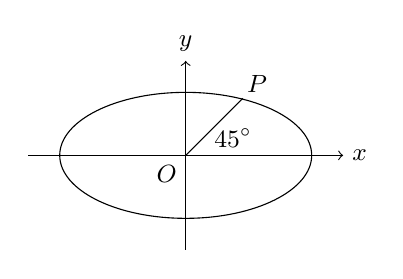
\begin{tikzpicture}[scale=.8]
            \begin{scope}\small
            \draw[->] (0,-1.5) to (0,1.5) node[above] {$y$};
            \draw[->] (-2.5,0) to (2.5,0) node[right] {$x$};
            \node (vO) at (-.3,-.3) {$O$};
            %\draw[smooth,samples=100,domain=.5:2.5] (plot(\x,{2.3*sqrt(\x-.5)});
            \draw (0,0) to (45:1.28);
            \node (vP) at (45:1.6) {$P$};
            \node (vP) at (20:.8) {$45^{\circ}$};
            \draw[smooth,samples=100] (0,0) ellipse (2cm and 1cm) ;
            \end{scope}
            \end{tikzpicture}
        \end{QBODY}
        \begin{QFROMS}
        \end{QFROMS}
        \begin{QTAGS}\QTAG{B4C4二次曲線}\QTAG{B4C4-2橢圓}\QTAG{圖形}\end{QTAGS}
        \begin{QANS}
            (2)
        \end{QANS}
        \begin{QSOLLIST}
        \end{QSOLLIST}
        \begin{QEMPTYSPACE}
        \end{QEMPTYSPACE}
    \end{QUESTION}
\end{QUESTIONS}
\begin{QUESTIONS}
    \begin{QUESTION}
        \begin{ExamInfo}{91}{學測}{多選}{7}
        \end{ExamInfo}
        \begin{ExamAnsRateInfo}{75}{93}{82}{50}
        \end{ExamAnsRateInfo}
        \begin{QBODY}
            若實數 $a,b,c$ 滿足 $abc>0$, $ab+bc+ca<0$, $a+b+c>0$, $a>b>c$ ,則下列選項何者為真? 
            \begin{QOPS} 
                \QOP $a>0$ 
                \QOP $b>0$ 
                \QOP $c>0$
                \QOP $|a|>|b|$ 
                \QOP $a^2>c^2$
            \end{QOPS}
        \end{QBODY}
        \begin{QFROMS}
        \end{QFROMS}
        \begin{QTAGS}\QTAG{B1C1數與式}\end{QTAGS}
        \begin{QANS}
            (1)(4)(5)
        \end{QANS}
        \begin{QSOLLIST}
        \end{QSOLLIST}
        \begin{QEMPTYSPACE}
        \end{QEMPTYSPACE}
    \end{QUESTION}
    \begin{QUESTION}
        \begin{ExamInfo}{91}{學測}{多選}{8}
        \end{ExamInfo}
        \begin{ExamAnsRateInfo}{60}{88}{64}{28}
        \end{ExamAnsRateInfo}
        \begin{QBODY}
            一機器狗每秒鐘前進或者後退一步,程式設計師讓機器狗以前進 $3$ 步,然後再後退 $2$ 步的規律移動。如果將此機器狗放在數線的原點,面向正的方向,以 $1$ 步的距離為 $1$ 單位長。令 $P(n)$ 表示第 $n$ 秒時機器狗所在位置的坐標,且 $P(0)=0$。那麼下列選項何者為真? 
            \begin{QOPS}
                \QOP $P(3)=3$ 
                \QOP $P(5)=1$ 
                \QOP $P(10)=2$
                \QOP $P(101)=21$ 
                \QOP $P(103)<P(104)$
            \end{QOPS}
        \end{QBODY}
        \begin{QFROMS}
        \end{QFROMS}
        \begin{QTAGS}\QTAG{B2C1數列級數}\QTAG{特殊數列}\QTAG{B2C1-1數列}\end{QTAGS}
        \begin{QANS}
            (1)(2)(3)(4)
        \end{QANS}
        \begin{QSOLLIST}
        \end{QSOLLIST}
        \begin{QEMPTYSPACE}
        \end{QEMPTYSPACE}
    \end{QUESTION}
    \begin{QUESTION}
        \begin{ExamInfo}{91}{學測}{多選}{9}
        \end{ExamInfo}
        \begin{ExamAnsRateInfo}{31}{53}{26}{14}
        \end{ExamAnsRateInfo}
        \begin{QBODY}
            下列哪些選項與方程組 $\left\{ \begin{array}{l} 2x+y+3z=0 \\ 4x+3y+6z =0 \end{array}\right.$ 的解集合相同?
            
            \begin{QOPS} 
                \QOP $y=0$ 
                
                \QOP 
                $\left\{ \begin{array}{l} 2x+3z=0 \\y=0 \end{array}\right.$
                
                \QOP
                $x=y=0$
                
                \QOP
                $\left\{ \begin{array}{l} x+\frac{1}{2}y+\frac{3}{2}z=0 \\ 4x+3y+6z =0 \end{array}\right.$
                
                \QOP
                $\left\{ \begin{array}{l} 6x+4y+9z=0 \\ 2x+y+3z =0 \end{array}\right.$
            \end{QOPS}
        \end{QBODY}
        \begin{QFROMS}
        \end{QFROMS}
        \begin{QTAGS}\QTAG{B4C3矩陣}\QTAG{B4C3-1線性方程組與矩陣}\QTAG{方程組}\end{QTAGS}
        \begin{QANS}
            (2)(4)(5)
        \end{QANS}
        \begin{QSOLLIST}
        \end{QSOLLIST}
        \begin{QEMPTYSPACE}
        \end{QEMPTYSPACE}
    \end{QUESTION}
    \begin{QUESTION}
        \begin{ExamInfo}{91}{學測}{多選}{10}
        \end{ExamInfo}
        \begin{ExamAnsRateInfo}{20}{40}{11}{9}
        \end{ExamAnsRateInfo}
        \begin{QBODY}
            觀察相關的函數圖形,判斷下列選項何者為真?
            \begin{QOPS}
                \QOP $10^x=x$ 有實數解 
                \QOP $10^x=x^2$ 有實數解 
                \QOP $x$ 為實數時,$10^x>x$ 恆成立 
                \QOP $x>0$ 時,$10^x>x^2$ 恆成立 
                \QOP $10^x= -x$ 有實數解
            \end{QOPS}
        \end{QBODY}
        \begin{QFROMS}
        \end{QFROMS}
        \begin{QTAGS}\QTAG{圖形}\QTAG{B1C3-2指數函數}\QTAG{B1C3指對數函數}\end{QTAGS}
        \begin{QANS}
            (2)(3)(4)(5)
        \end{QANS}
        \begin{QSOLLIST}
        \end{QSOLLIST}
        \begin{QEMPTYSPACE}
        \end{QEMPTYSPACE}
    \end{QUESTION}
    \begin{QUESTION}
        \begin{ExamInfo}{91}{學測}{多選}{11}
        \end{ExamInfo}
        \begin{ExamAnsRateInfo}{16}{30}{12}{6}
        \end{ExamAnsRateInfo}
        \begin{QBODY}
            某甲自 $89$ 年 $7$ 月起,每月 $1$ 日均存入銀行 $1000$ 元,言明以月利率 $0.5\%$ 按月複利計息,到 $90$ 年 $7$ 月 $1$ 日提出。某乙則於 $89$ 年 $7$ 月起,每單月(一月、三月、五月 $\cdots$) 1 日均存入 銀行 $2000$ 元,亦以月利率 $0.5\%$ 按月複利計息,到 $90$ 年 $7$ 月 $1$ 日提出。一整年中,兩人都存 入本金 $12000$ 元。提出時,甲得本利和 $A$ 元,乙得本利和 $B$ 元。問下列選項何者為真? 
            \begin{QOPS} 
                \QOP $B>A$ 
                \QOP $A= 1000\cdot [\Sum_{k=1}^{12} (1.005)^k ]$ 
                \QOP $B= 2000 [\Sum_{k=1}^{6} (1.005)^{2k}] $ 
                \QOP $A< 12000 (1.005)^{12}$  
                \QOP $B< 12000 (1.005)^{12}$
            \end{QOPS}
        \end{QBODY}
        \begin{QFROMS}
        \end{QFROMS}
        \begin{QTAGS}\QTAG{B2C1數列級數}\QTAG{B2C1-2級數}\QTAG{複利}\end{QTAGS}
        \begin{QANS}
            (1)(2)(3)(4)(5)
        \end{QANS}
        \begin{QSOLLIST}
        \end{QSOLLIST}
        \begin{QEMPTYSPACE}
        \end{QEMPTYSPACE}
    \end{QUESTION}
    \begin{QUESTION}
        \begin{ExamInfo}{91}{學測}{多選}{12}
        \end{ExamInfo}
        \begin{ExamAnsRateInfo}{36}{67}{29}{12}
        \end{ExamAnsRateInfo}
        \begin{QBODY}
            在 $\triangle ABC$ 中,下列哪些選項的條件有可能成立?
            \begin{QOPS} 
                \QOP $\sin A=\sin B= \sin C= \frac{\sqrt{3}}{2}$ 
                \QOP $\sin A$, $\sin B$, $\sin C$ 均小於 $\frac{1}{2}$ 
                \QOP $\sin A, \sin B$, $\sin C$ 均大於 $\frac{\sqrt{3}}{2}$ 
                \QOP $\sin A = \sin B = \sin C =\frac{1}{2}$ 
                \QOP $\sin A= \sin B= \frac{1}{2}$ , $\sin C= \frac{\sqrt{3}}{2}$
            \end{QOPS}
        \end{QBODY}
        \begin{QFROMS}
        \end{QFROMS}
        \begin{QTAGS}\QTAG{B3C1-3正弦定理與餘弦定理}\QTAG{B3C1三角}\end{QTAGS}
        \begin{QANS}
            (1)(2)(5)
        \end{QANS}
        \begin{QSOLLIST}
        \end{QSOLLIST}
        \begin{QEMPTYSPACE}
        \end{QEMPTYSPACE}
    \end{QUESTION}
\end{QUESTIONS}
\begin{QUESTIONS}
    \begin{QUESTION}
        \begin{ExamInfo}{91}{學測}{填充}{A}
        \end{ExamInfo}
        \begin{ExamAnsRateInfo}{28}{65}{17}{2}
        \end{ExamAnsRateInfo}
        \begin{QBODY}
            工匠在窗子外邊想做一個圓弧型的花台,
            此花台在窗口的中央往外伸出 72 公分,
            窗口的寬度是 168 公分,
            則此圓弧的圓半徑為 
            \TCNBOX{\TCN\TCN} 公分。
        \end{QBODY}
        \begin{QFROMS}
        \end{QFROMS}
        \begin{QTAGS}\QTAG{B3C2-3圓與直線的關係}\QTAG{B3C2直線與圓}\end{QTAGS}
        \begin{QANS}
            $85$
        \end{QANS}
        \begin{QSOLLIST}
        \end{QSOLLIST}
        \begin{QEMPTYSPACE}
        \end{QEMPTYSPACE}
    \end{QUESTION}
    \begin{QUESTION}
        \begin{ExamInfo}{91}{學測}{填充}{B}
        \end{ExamInfo}
        \begin{ExamAnsRateInfo}{50}{70}{51}{29}
        \end{ExamAnsRateInfo}
        \begin{QBODY}
            $2^{20}-1$ 與 $2^{19}+1$ 的最大公因數為 
            \TCNBOX{\TCN}
        \end{QBODY}
        \begin{QFROMS}
        \end{QFROMS}
        \begin{QTAGS}\QTAG{B1C1數與式}\end{QTAGS}
        \begin{QANS}
            $3$
        \end{QANS}
        \begin{QSOLLIST}
        \end{QSOLLIST}
        \begin{QEMPTYSPACE}
        \end{QEMPTYSPACE}
    \end{QUESTION}
    \begin{QUESTION}
        \begin{ExamInfo}{91}{學測}{填充}{C}
        \end{ExamInfo}
        \begin{ExamAnsRateInfo}{38}{70}{32}{12}
        \end{ExamAnsRateInfo}
        \begin{QBODY}
            某公司民國 $85$ 年營業額為 $4$ 億元,民國 $86$ 年營業額為 $6$ 億元,該年的成長率為 $50\%$。 $87$、$88$、$89$ 三年的成長率皆相同,且民國 $89$ 年的營業額為 48 億元。則該公司 89 年的成長率為 
            $\TCNBOX{\TCN\TCN\TCN} \%$
        \end{QBODY}
        \begin{QFROMS}
        \end{QFROMS}
        \begin{QTAGS}\QTAG{B2C4-1一維數據分析}\QTAG{幾何平均數}\QTAG{B2C4數據分析}\end{QTAGS}
        \begin{QANS}
            $100\%$
        \end{QANS}
        \begin{QSOLLIST}
        \end{QSOLLIST}
        \begin{QEMPTYSPACE}
        \end{QEMPTYSPACE}
    \end{QUESTION}
    \begin{QUESTION}
        \begin{ExamInfo}{91}{學測}{填充}{D}
        \end{ExamInfo}
        \begin{ExamAnsRateInfo}{50}{67}{53}{30}
        \end{ExamAnsRateInfo}
        \begin{QBODY}
            在一個圓的圓周上,平均分佈了 $60$ 個洞,兩洞間稱為一間隔。在 $A$ 洞打上一支木樁並綁上線,然後依逆時針方向前進每隔 $9$ 個間隔就再打一支木樁,並綁上線,依此繼續操作,如右圖所示。 試問輪回到 $A$ 洞需再打樁前,總共已經打了$\TCNBOX{{\TCN\TCN}}$支木樁。\\
            
            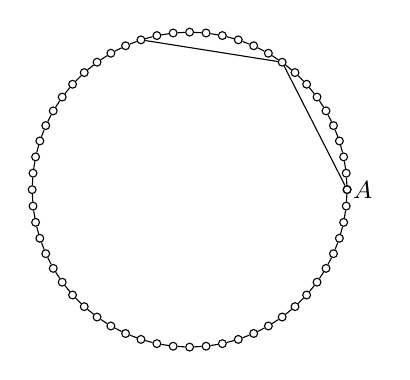
\begin{tikzpicture}[scale=.4]
            \begin{scope}
            \foreach \i in {0,1,2,...,59,60}
            \node[draw,circle,inner sep=1pt]  (v\i) at (6*\i:5) {};
            \foreach \i [remember=\i as \lasti (initially 0)] in {1,2,...,60}
            \draw (v\i) to (v\lasti);
            \draw (v0) to (v9);
            \draw (v9) to (v18);
            \node at (5.5,0) {\small $A$};
            \end{scope}
            \end{tikzpicture}
        \end{QBODY}
        \begin{QFROMS}
        \end{QFROMS}
        \begin{QTAGS}\QTAG{不是99課綱}\end{QTAGS}
        \begin{QANS}
            $20$
        \end{QANS}
        \begin{QSOLLIST}
        \end{QSOLLIST}
        \begin{QEMPTYSPACE}
        \end{QEMPTYSPACE}
    \end{QUESTION}
    \begin{QUESTION}
        \begin{ExamInfo}{91}{學測}{填充}{E}
        \end{ExamInfo}
        \begin{ExamAnsRateInfo}{41}{70}{41}{12}
        \end{ExamAnsRateInfo}
        \begin{QBODY}
            某次網球比賽共有 $128$ 位選手參加,採單淘汰制,每輪淘汰一半的選手,剩下一半的選手進入下一輪。在第 $1$ 輪被淘汰的選手可獲得 $1$ 萬元,在第 $2$ 輪被淘汰的選手可獲得 $2$ 萬元,在第 $k$ 輪被淘汰的選手可獲得 $2^{k-1}$ 萬元,而冠軍則可獲得 $128$ 萬元。試問全部比賽獎金共$\TCNBOX{\TCN\TCN\TCN}$萬元。
        \end{QBODY}
        \begin{QFROMS}
        \end{QFROMS}
        \begin{QTAGS}\QTAG{B2C1數列級數}\QTAG{B2C1-2級數}\QTAG{等比級數}\end{QTAGS}
        \begin{QANS}
            $576$萬元
        \end{QANS}
        \begin{QSOLLIST}
        \end{QSOLLIST}
        \begin{QEMPTYSPACE}
        \end{QEMPTYSPACE}
    \end{QUESTION}
    \begin{QUESTION}
        \begin{ExamInfo}{91}{學測}{填充}{F}
        \end{ExamInfo}
        \begin{ExamAnsRateInfo}{51}{89}{50}{14}
        \end{ExamAnsRateInfo}
        \begin{QBODY}
            某人隔河測一山高,在 $A$ 點觀測山時,山的方位為東偏北 $60^\circ$,
            山頂的仰角為 $45^\circ$,
            某人自 $A$ 點向東行 $600$ 公尺到達 $B$ 點,山的方位變成在西偏北 $60^\circ$,則山有多高? 答: $
            \TCNBOX{\TCN\TCN\TCN}$ 公尺。
        \end{QBODY}
        \begin{QFROMS}
        \end{QFROMS}
        \begin{QTAGS}\QTAG{B3C1-5三角測量}\QTAG{B3C1三角}\end{QTAGS}
        \begin{QANS}
            $600$
        \end{QANS}
        \begin{QSOLLIST}
        \end{QSOLLIST}
        \begin{QEMPTYSPACE}
        \end{QEMPTYSPACE}
    \end{QUESTION}
    \begin{QUESTION}
        \begin{ExamInfo}{91}{學測}{填充}{G}
        \end{ExamInfo}
        \begin{ExamAnsRateInfo}{29}{58}{24}{5}
        \end{ExamAnsRateInfo}
        \begin{QBODY}
            有一群體有九位成員,其身高分別為(單位:公分) $160, 163, 166, 170, 172, 174, 176, 178, 180$ , 此九人的平均身高為 $171$ 公分。今隨機抽樣 $3$ 人,則抽到 $3$ 人的平均身高等於母體平均身高的機率為 
            $\TCNBOX{\FR{\TCN}{\TCN\TCN}} $。
        \end{QBODY}
        \begin{QFROMS}
        \end{QFROMS}
        \begin{QTAGS}\QTAG{平均數}\QTAG{B2C4-1一維數據分析}\QTAG{B2C3機率}\QTAG{B2C3-2機率的定義與性質}\QTAG{B2C4數據分析}\end{QTAGS}
        \begin{QANS}
            $\frac{1}{28}$
        \end{QANS}
        \begin{QSOLLIST}
        \end{QSOLLIST}
        \begin{QEMPTYSPACE}
        \end{QEMPTYSPACE}
    \end{QUESTION}
    \begin{QUESTION}
        \begin{ExamInfo}{91}{學測}{填充}{H}
        \end{ExamInfo}
        \begin{ExamAnsRateInfo}{28}{69}{14}{1}
        \end{ExamAnsRateInfo}
        \begin{QBODY}
            右圖為一正立方體,被一平面截出一個四邊形 $ABCD$,
            其中 $B,D$ 分別為稜的中點,
            且 $\overline{EA}: \overline{AF}=1:2$,則 $\cos\angle DAB= $ 
            $\TCNBOX{\FR{\TCN}{\TCN\TCN}}$
            
            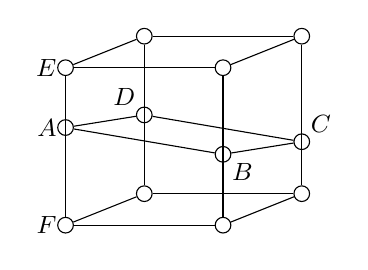
\begin{tikzpicture}
                \small
                \tikzstyle{vnode}=[draw,circle,inner sep =2pt];
                \node[vnode] (v000) at (0,0) {};
                \node[anchor =east] (t000) at (v000) {};
                \node[vnode] (v001) at (0,2) {};
                \node[anchor =east] (t000) at (v001) {};
                \node[vnode] (v011) at (2,2) {};
                \node[anchor =west] (t011) at (v011) {};
                \node[vnode] (v010) at (2,0) {};
                \node[anchor =west] (t010) at (v010) {};
                \node[vnode] (v100) at (-1.0,-.4) {};
                \node[anchor =east] (t100) at (v100) {$F$};
                \node[vnode] (v101) at (-1.0,1.6) {};
                \node[anchor =east] (t101) at (v101) {$E$};
                \node[vnode] (v111) at (1.0,1.6) {};
                \node[anchor =north east] (t111) at (v111) {};
                \node[vnode] (v110) at (1.0,-0.4) {};
                \node[anchor =west] (t110) at (v110) {};
                \node[vnode] (vA) at (-1,.84) {};
                \node[anchor =east] (tA) at (vA) {$A$};
                \node[vnode] (vC) at (2,.66) {};
                \node[anchor =south west] (tC) at (vC) {$C$};
                \node[vnode] (vD) at (0,1) {};
                \node[anchor =south east] (tD) at (vD) {$D$};
                \node[vnode] (vB) at (1,.5) {};
                \node[anchor =north west] (tB) at (vB) {$B$};
                \draw (vD) to[dashed] (vA);
                \draw (vD) to[dashed] (vC);
                \draw (vB) to (vA);
                \draw (vB) to (vC);
                \foreach \i in {01,10,11}{
                    \draw (v0\i) to (v1\i);
                    \draw (v\i  0) to (v\i 1);
                }
                \draw (v000) to[dashed] (v100);
                \draw (v000) to[dashed] (v010);
                \draw (v000) to[dashed] (v001);
                \draw (v001) to (v011);
                \draw (v100) to (v110);
                \draw (v101) to (v111);              
            \end{tikzpicture}
        \end{QBODY}
        \begin{QFROMS}
        \end{QFROMS}
        \begin{QTAGS}\QTAG{B4C1-3空間向量的內積}\QTAG{B4C1空間向量}\end{QTAGS}
        \begin{QANS}
            $\frac{1}{37}$
        \end{QANS}
        \begin{QSOLLIST}
        \end{QSOLLIST}
        \begin{QEMPTYSPACE}
        \end{QEMPTYSPACE}
    \end{QUESTION}
\end{QUESTIONS}
